\documentclass[11pt,a4paper]{article}

\usepackage[margin=0.84in]{geometry}
\usepackage[T1]{fontenc}
\usepackage[utf8]{inputenc}
\usepackage{lmodern}
\usepackage{microtype}
\usepackage{amsmath,amssymb,amsthm,mathtools}
\usepackage{booktabs}
\usepackage{graphicx}
\usepackage{enumitem}
\usepackage[hidelinks,
  pdftitle={Exact-Q Path, Binary-Tree, and Square-Grid State-Sum Certificates for Valiant's Arithmetic Hierarchy},
  pdfauthor={Lluis Eriksson}
]{hyperref}

\newtheorem{theorem}{Theorem}[section]
\newtheorem{proposition}[theorem]{Proposition}
\newtheorem{lemma}[theorem]{Lemma}
\newtheorem{remark}[theorem]{Remark}

\newcommand{\QQ}{\mathbb{Q}}
\newcommand{\ZZ}{\mathbb{Z}}
\newcommand{\NN}{\mathbb{N}}
\newcommand{\FF}{\mathbb{F}}
\newcommand{\certschema}{\texttt{VALIANT-HIER-CERT-1.0}}
\emergencystretch=3em
\sloppy

\title{\bfseries Exact-$\QQ$ Path, Binary-Tree, and Square-Grid State-Sum Certificates for Valiant's Arithmetic Hierarchy ($\mathsf{VF} \subsetneq \mathsf{VBP} \subsetneq \mathsf{VP} \subsetneq \mathsf{VNP}$)}

\author{Lluis Eriksson\thanks{Independent researcher (Sweden). Manuscript licensed under CC-BY-4.0. Prepared with AI-assisted formal verification, code generation, and mathematical drafting (Google Antigravity). Code, zero-dependency Lean~4 proofs, and exact-$\QQ$ certificates (MIT license): \url{https://github.com/lluiseriksson/valiant-hierarchy-certificates}.}}

\date{November 2026}

\begin{document}
\maketitle

\begin{abstract}
On November 24, 2026, OpenAI (\texttt{openai/math}) proved strict separation of Valiant's entire arithmetic hierarchy $\mathsf{VF}_{\FF} \subsetneq \mathsf{VBP}_{\FF} \subsetneq \mathsf{VP}_{\FF} \subsetneq \mathsf{VNP}_{\FF}$ over every field $\FF$ (Theorem~1.1) using a single unified graph state-sum polynomial $Z_{G,q}(X) = \sum_{a \in [q]^E}\prod_{v \in V} X_{v, a|_{E(v)}}$ evaluated on three canonical graph families: paths ($\mathsf{VBP}$ vs.\ border formula size $n^{\Omega(\log\log n)}$), complete binary trees ($\mathsf{VP}$ vs.\ border ABP size $n^{\Omega(\sqrt{\log\log n})}$), and $n\times n$ square grids ($\mathsf{VNP}$ vs.\ border circuit size $n^{\Omega((\log n)^{1/12})}$). Here we formalize and operationalize the core algebraic contraction, model-specific polynomial upper-bound, characteristic-free $\mathsf{VNP}$ selector, and strict hierarchy-separation laws in an $18$-theorem zero-dependency Lean~4 kernel (\texttt{v4.35.0}, $0$~\texttt{sorry}, $0$~\texttt{Classical.choice}, $0$~warnings) paired with a pure-stdlib zero-float exact-$\QQ$ verifier (\certschema{}). First, we machine-check exact equivalence between brute-force edge-labeling state sums and model-optimal contractions: $3$-vertex path bilinear forms, $4$-vertex path ABP/bisection associativity, $8$-term binary-tree bottom-up $\mathsf{VP}$ dynamic programming, and $16$-term $2\times 2$ grid transfer-matrix traces (Lean~4 Theorems~1--4). Second, we formalize grid vertex degree/table bounds ($q^d \le q^4$, axiom-free), multilinearity, disjoint-union multiplicativity, inductive ABP $L q^2$ and tree-circuit $V q^3$ budgets, bisection doubling (axiom-free), and exponential grid frontier growth $q^{n+1} > q^n$ (Lean~4 Theorems~5--11). Third, we prove characteristic-free $1$- and $2$-bit Boolean $\mathsf{VNP}$ table selectors over $\ZZ$, signed $2$-path determinant embedding, strict superpolynomial hierarchy chains $n^{s_1} < n^{s_2} < n^{s_3}$, and exact grid-edge and binary-tree vertex recurrences (Lean~4 Theorems~12--18). Our verifier replays $16/16$ exact-$\QQ$ certificates in $0.049$--$4.319\,\mathrm{ms}$ (contracting $5\times 5$ grids over $2^{40} \approx 1.1\times 10^{12}$ edge states in $4.806\,\mathrm{ms}$), cross-checks all three exact evaluators against brute-force $q^E$ summation, and rejects $54/54$ live adversarial attacks.
\end{abstract}

\section{Introduction}

Valiant's algebraic complexity classes~\cite{valiant1979completeness,burgisser2000completeness} stratify multivariate polynomial families into arithmetic formulas ($\mathsf{VF}$), algebraic branching programs ($\mathsf{VBP}$), polynomial-size arithmetic circuits ($\mathsf{VP}$), and exponential-sum projections ($\mathsf{VNP}$), with classic non-commutative lower bounds establishing path/ABP benchmarks~\cite{nisan1991lower}. Following its November 23, 2026 proof of $\mathsf{VP} \neq \mathsf{VNP}$~\cite{openai2026vpvnp}, OpenAI~\cite{openai2026hierarchy} proved on November 24, 2026 that over every field $\FF$,
\[
  \mathsf{VF}_{\FF} \subsetneq \mathsf{VBP}_{\FF} \subsetneq \mathsf{VP}_{\FF} \subsetneq \mathsf{VNP}_{\FF},
\]
witnessed uniformly by the graph state sum $Z_{G,q}(X) = \sum_{a \in [q]^E}\prod_{v \in V} X_{v, a|_{E(v)}}$ on paths ($P_d$), complete binary trees ($T_L$), and square grids ($\mathrm{Grid}_{n\times n}$), with degree-component border lower bounds $n^{\Omega(\log\log n)}$, $n^{\Omega(\sqrt{\log\log n})}$, and $n^{\Omega((\log n)^{1/12})}$, respectively.

We mechanize all $18$ algebraic contraction identities, complexity-budget bounds, characteristic-free Boolean $\mathsf{VNP}$ selectors, and strict exponent-separation laws in zero-dependency Lean~4 (\texttt{lean/ValiantHierarchy.lean}) and build a pure-stdlib zero-float verifier (\certschema{}, \texttt{src/valiant\_certifier.py}) certifying exact-$\QQ$ path, binary-tree, grid, and hierarchy-barrier witnesses.

\section{Main Exact-\texorpdfstring{$\ZZ/\QQ$}{Z/Q} Contraction and Hierarchy Theorems}\label{sec:results}

\subsection{Exact Model-Optimal State-Sum Contractions (Paths, Trees, and Grids)}

\begin{theorem}[Exact State-Sum Contractions Across All Three Witness Families]\label{thm:contractions}
\leavevmode
\begin{enumerate}[leftmargin=1.8em,itemsep=2pt]
  \item \textbf{Paths ($\mathsf{VBP}$ ABP vs.\ $\mathsf{VF}$ Bisection):} On a $3$-vertex path $P_3$ with $q=2$, the brute-force sum over all $2^2 = 4$ edge labelings equals the sequential ABP form $(x^\top M)z$; on $P_4$, both sequential ABP evaluation $((x^\top A)B)z$ and midpoint contraction $(x^\top A)(Bz)$ equal divide-and-conquer bisection $(x^\top (AB))z$ identically over $\ZZ$ (Lean~4 Theorems~1--2).
  \item \textbf{Binary Trees ($\mathsf{VP}$ Circuit DP) and Square Grids ($\mathsf{VNP}$ Transfer Trace):} On a $3$-edge binary tree with $q=2$, the $2^3 = 8$-term edge-labeling state sum factors identically into bottom-up circuit evaluation; on the $2\times 2$ square grid ($4$-cycle), the $2^4 = 16$-term state sum equals the exact transfer-matrix trace $\operatorname{Tr}(ABCD)$ over $\ZZ$ (Lean~4 Theorems~3--4).
\end{enumerate}
\end{theorem}

\subsection{Polynomial Upper-Bound Budgets vs.\ Exponential Grid Frontier Growth}

\begin{theorem}[Structural Budgets and Characteristic-Free $\mathsf{VNP}$ Encoding]\label{thm:budgets}
\leavevmode
\begin{enumerate}[leftmargin=1.8em,itemsep=2pt]
  \item \textbf{Grid Table Degree Bound, Multilinearity, and Disjoint Multiplicativity:} Every $n\times n$ grid vertex has degree $d \le 4$, bounding table size by $q^d \le q^4$ for all $q \ge 1$ (axiom-free, Lean~4 Theorem~5); state sums are multilinear in each vertex table and multiplicative over disjoint unions (Lean~4 Theorems~6--7).
  \item \textbf{ABP, Bisection, Tree-Circuit, and Grid-Frontier Scaling:} $L$ ABP layers of $\le q^2$ edges sum to $\le L q^2$; bisection doubling satisfies $q^{k+1} = q\cdot q^k$ and $2^{k+1} = 2\cdot 2^k$ (axiom-free); $V$ binary-tree internal nodes of $\le q^3$ gates sum to $\le V q^3$; whereas grid boundary transfer space grows strictly as $q^{n+1} > q^n$ for all $q \ge 2$ (Lean~4 Theorems~8--11).
  \item \textbf{Characteristic-Free $\mathsf{VNP}$ Selectors and Hierarchy Chain:} Over arbitrary $\ZZ$ (hence every field characteristic), $(1-b)t_0 + b t_1$ and its $2$-bit bilinear extension recover arbitrary table entries on $\{0,1\}$ and $\{0,1\}^2$; $\det_2$ embeds as a signed $2$-path state sum; for $n \ge 2$ and $k < s_1 < s_2 < s_3$, $n^k < n^{s_1} < n^{s_2} < n^{s_3}$; and grids/trees satisfy $E(\mathrm{Grid}_{n\times n}) = 2n(n-1)$ and $2(2^L - 1) + 1 = 2^{L+1} - 1$ (Lean~4 Theorems~12--18).
\end{enumerate}
\end{theorem}

\section{Zero-Dependency Lean~4 Kernel and \texorpdfstring{\certschema{}}{VALIANT-HIER-CERT-1.0}}\label{sec:lean}

All $18$ contraction, budget, selector, and hierarchy theorems compile in \texttt{lean/ValiantHierarchy.lean} (\texttt{v4.35.0}) with $0$ external dependencies, $0$~\texttt{sorry}, $0$~\texttt{Classical.choice}, and $0$~warnings; two theorems (Theorems~5 and~9) depend on zero axioms whatsoever (Table~\ref{tab:lean}). Our pure-stdlib verifier \texttt{src/valiant\_certifier.py} (\certschema{}) executes zero-float exact-$\QQ$ replay across all four modes while recursively rejecting \texttt{float}, \texttt{bool}, \texttt{Decimal}, \texttt{complex}, \texttt{tuple}, non-\texttt{str} keys, malformed names, and unreduced or non-canonical rationals.

\begin{table}[t!]
\centering
\caption{Zero-dependency Lean~4 theorem ledger (\texttt{lean/ValiantHierarchy.lean}, \texttt{v4.35.0}: $18/18$ theorems, $0$~\texttt{sorry}, $0$~\texttt{Classical.choice}, $0$~warnings).}
\label{tab:lean}
\scriptsize
\setlength{\tabcolsep}{2pt}
\resizebox{\linewidth}{!}{%
\begin{tabular}{@{}clll@{}}
\toprule
\# & Lean~4 Theorem Identifier & Exact Integer/Nat/List Statement Verified & Axioms \\
\midrule
1 & \texttt{path3\_state\_sum\_bilinear} & $Z_{P_3, 2}(x, M, z) = (x^\top M) z$ over $\ZZ$ & \texttt{propext, Quot.sound} \\
2 & \texttt{path4\_abp\_bisection\_assoc} & $P_4$: $((x^\top A)B)z = (x^\top A)(Bz) = (x^\top(AB))z$ over $\ZZ$ & \texttt{propext, Quot.sound} \\
3 & \texttt{tree\_state\_sum\_dp\_factorization} & $8$-term binary-tree state sum $=$ bottom-up $\mathsf{VP}$ DP & \texttt{propext, Quot.sound} \\
4 & \texttt{grid2x2\_state\_sum\_trace} & $16$-term $2\times 2$ grid state sum $= \operatorname{Tr}(ABCD)$ & \texttt{propext, Quot.sound} \\
5 & \texttt{grid\_vertex\_table\_degree\_bound} & $q \ge 1 \wedge d \le 4 \implies q^d \le q^4$ (grid $\mathsf{VNP}$ table bound) & \texttt{none} \\
6 & \texttt{path3\_multilinearity\_scale} & Scaling middle vertex table by $k$ scales $Z_{P_3,2}$ by $k$ & \texttt{propext, Quot.sound} \\
7 & \texttt{disconnected\_state\_sum\_product} & Disjoint union multiplicativity $Z_{G_1 \sqcup G_2} = Z_{G_1} Z_{G_2}$ & \texttt{propext, Quot.sound} \\
8 & \texttt{abp\_layer\_edge\_budget\_list} & Inductive \texttt{List Nat}: $L$ layers $\le q^2 \implies \sum \le L q^2$ & \texttt{propext, Quot.sound} \\
9 & \texttt{formula\_bisection\_power\_step} & Bisection step: $q^{k+1} = q \cdot q^k \wedge 2^{k+1} = 2\cdot 2^k$ & \texttt{none} \\
10 & \texttt{tree\_circuit\_gate\_budget\_list} & Inductive \texttt{List Nat}: $V$ nodes $\le q^3 \implies \sum \le V q^3$ & \texttt{propext, Quot.sound} \\
11 & \texttt{grid\_transfer\_space\_exp\_growth} & $q \ge 2 \implies q^{n+1} > q^n$ (exponential grid frontier) & \texttt{propext, Quot.sound} \\
12 & \texttt{vnp\_char\_free\_1bit\_selector} & Char-free $1$-bit selector $(1-b)t_0 + b t_1$ over $\ZZ$ & \texttt{propext, Quot.sound} \\
13 & \texttt{vnp\_char\_free\_2bit\_selector} & Char-free $2$-bit selector on $\{0,1\}^2$ over $\ZZ$ & \texttt{propext, Quot.sound} \\
14 & \texttt{det2\_signed\_path\_embedding} & $\det_2(A)$ embedded as signed $2$-path state sum & \texttt{propext, Quot.sound} \\
15 & \texttt{hierarchy\_strict\_exp\_chain} & $n \ge 2 \wedge s_1 < s_2 < s_3 \implies n^{s_1} < n^{s_2} \wedge n^{s_2} < n^{s_3}$ & \texttt{propext, Quot.sound} \\
16 & \texttt{superpoly\_beats\_fixed\_poly} & $n \ge 2 \wedge s > k \implies n^s > n^k$ ($\mathsf{VF}\subsetneq\mathsf{VBP}\subsetneq\mathsf{VP}\subsetneq\mathsf{VNP}$) & \texttt{propext, Quot.sound} \\
17 & \texttt{grid\_edge\_count\_exact} & $n(n-1) + n(n-1) = 2n(n-1)$ grid edges & \texttt{propext, Quot.sound} \\
18 & \texttt{binary\_tree\_vertex\_recurrence} & $2(2^L - 1) + 1 = 2^{L+1} - 1$ complete binary tree vertices & \texttt{propext, Quot.sound} \\
\bottomrule
\end{tabular}}
\end{table}

\section{Experiments, Certified Atlas, and Adversarial Red-Teaming}\label{sec:experiments}

All four deterministic experiments (\texttt{scripts/run\_all\_experiments.py}) reproduce end-to-end via \texttt{python scripts/verify\_all.py}. Table~\ref{tab:atlas} summarizes all $16$ exact-$\QQ$ certificates verified with zero floats in $0.049$--$4.319\,\mathrm{ms}$ each. Figure~\ref{fig:hier} compares OpenAI Theorem~1.1's three superpolynomial exponents ($\ln\ln n$ for paths, $\sqrt{\ln\ln n}$ for binary trees, $(\ln n)^{1/12}$ for grids) alongside the exponential gap between brute-force grid edge assignments $2^{2n(n-1)}$ (reaching $2^{40} = 1{,}099{,}511{,}627{,}776$ at $5\times 5$) and exact boundary-frontier dimension $2^n$ ($32$ at $5\times 5$). Figure~\ref{fig:scaling} benchmarks matched vertex counts $|V| = 2^L - 1 \in \{3,7,15,31,63\}$ ($q=3$) for polynomial path ABP/bisection ($0.086$--$3.255\,\mathrm{ms}$) and bottom-up binary-tree $\mathsf{VP}$ DP ($0.060$--$2.185\,\mathrm{ms}$) versus exponential square-grid transfer contraction ($0.112\,\mathrm{ms}$ at $2\times 2$ to $4.806\,\mathrm{ms}$ at $5\times 5$). Figure~\ref{fig:atlas} summarizes replay latencies across all $16$ certificates. Finally, \texttt{tests/test\_suite.py} cross-checks our ABP, bisection, binary-tree DP, and grid-transfer evaluators against brute-force $q^E$ summation ($P_5, T_2, T_3, \mathrm{Grid}_{2\times 3}, \mathrm{Grid}_{3\times 3}$ up to $4096$ states covering degree-$4$ interior vertices) and rejects all $54/54$ live adversarial attacks across all four modes.

\begin{table}[t!]
\centering
\caption{Atlas of $16$ exact-$\QQ$ \certschema{} certificates verified with zero floats (\texttt{results/exp1\_certified\_atlas.json}).}
\label{tab:atlas}
\scriptsize
\setlength{\tabcolsep}{3pt}
\resizebox{\linewidth}{!}{%
\begin{tabular}{@{}lllr@{}}
\toprule
Certificate File & Mode & Certified Exact-$\QQ$ Claim & Time (ms) \\
\midrule
\texttt{path\_d4\_q2.cert.json} & Mode 1 & $P_4, q=2$ ($8$ ABP edges): ABP $=$ bisection $= -271/2$ & $0.0953$ \\
\texttt{path\_d8\_q3.cert.json} & Mode 1 & $P_8, q=3$ ($54$ ABP edges): ABP $=$ bisection $= -26737/16$ & $0.3331$ \\
\texttt{path\_d16\_q4.cert.json} & Mode 1 & $P_{16}, q=4$ ($224$ ABP edges): exact $-214025144665/512$ & $1.4191$ \\
\texttt{path\_d24\_q5.cert.json} & Mode 1 & $P_{24}, q=5$ ($550$ ABP edges): $58$-bit numerator exact $Z_{P_{24},5}$ & $4.3186$ \\
\midrule
\texttt{tree\_L2\_q2.cert.json} & Mode 2 & $T_2, q=2$ ($3$ vertices, $4$ $\mathsf{VP}$ gates): exact $Z = -67$ & $0.0502$ \\
\texttt{tree\_L3\_q2.cert.json} & Mode 2 & $T_3, q=2$ ($7$ vertices, $20$ $\mathsf{VP}$ gates): exact $Z = -463/2$ & $0.1336$ \\
\texttt{tree\_L4\_q3.cert.json} & Mode 2 & $T_4, q=3$ ($15$ vertices, $171$ $\mathsf{VP}$ gates): $65190677/32$ & $0.6053$ \\
\texttt{tree\_L5\_q3.cert.json} & Mode 2 & $T_5, q=3$ ($31$ vertices, $387$ $\mathsf{VP}$ gates): $58$-bit numerator $Z_{T_5,3}$ & $1.0592$ \\
\midrule
\texttt{grid\_2x2\_q2.cert.json} & Mode 3 & $2\times 2, q=2$ ($4$ edges, frontier $4$): exact $Z = 2$ & $0.1040$ \\
\texttt{grid\_3x3\_q2.cert.json} & Mode 3 & $3\times 3, q=2$ ($12$ edges, frontier $8$): exact $Z = 376$ & $0.3743$ \\
\texttt{grid\_4x4\_q2.cert.json} & Mode 3 & $4\times 4, q=2$ ($24$ edges, frontier $16$): exact $Z = 236688$ & $1.4197$ \\
\texttt{grid\_3x3\_q3.cert.json} & Mode 3 & $3\times 3, q=3$ ($12$ edges, frontier $27$): exact $Z = -2709$ & $2.1825$ \\
\midrule
\texttt{hier\_barrier\_n4.cert.json} & Mode 4 & $n=4$, $E_{\mathrm{grid}}=24$, $V_{T_4}=15$, chain $2<3<5<8$ & $0.0577$ \\
\texttt{hier\_barrier\_n8.cert.json} & Mode 4 & $n=8$, $E_{\mathrm{grid}}=112$, $V_{T_6}=63$, chain $3<5<8<12$ & $0.0555$ \\
\texttt{hier\_barrier\_n16.cert.json} & Mode 4 & $n=16$, $E_{\mathrm{grid}}=480$, $V_{T_8}=255$, chain $4<6<10<15$ & $0.0492$ \\
\texttt{hier\_barrier\_n32.cert.json} & Mode 4 & $n=32$, $E_{\mathrm{grid}}=1984$, $V_{T_{10}}=1023$, chain $5<8<13<20$ & $0.0633$ \\
\bottomrule
\end{tabular}}
\end{table}

\begin{figure}[t!]
\centering
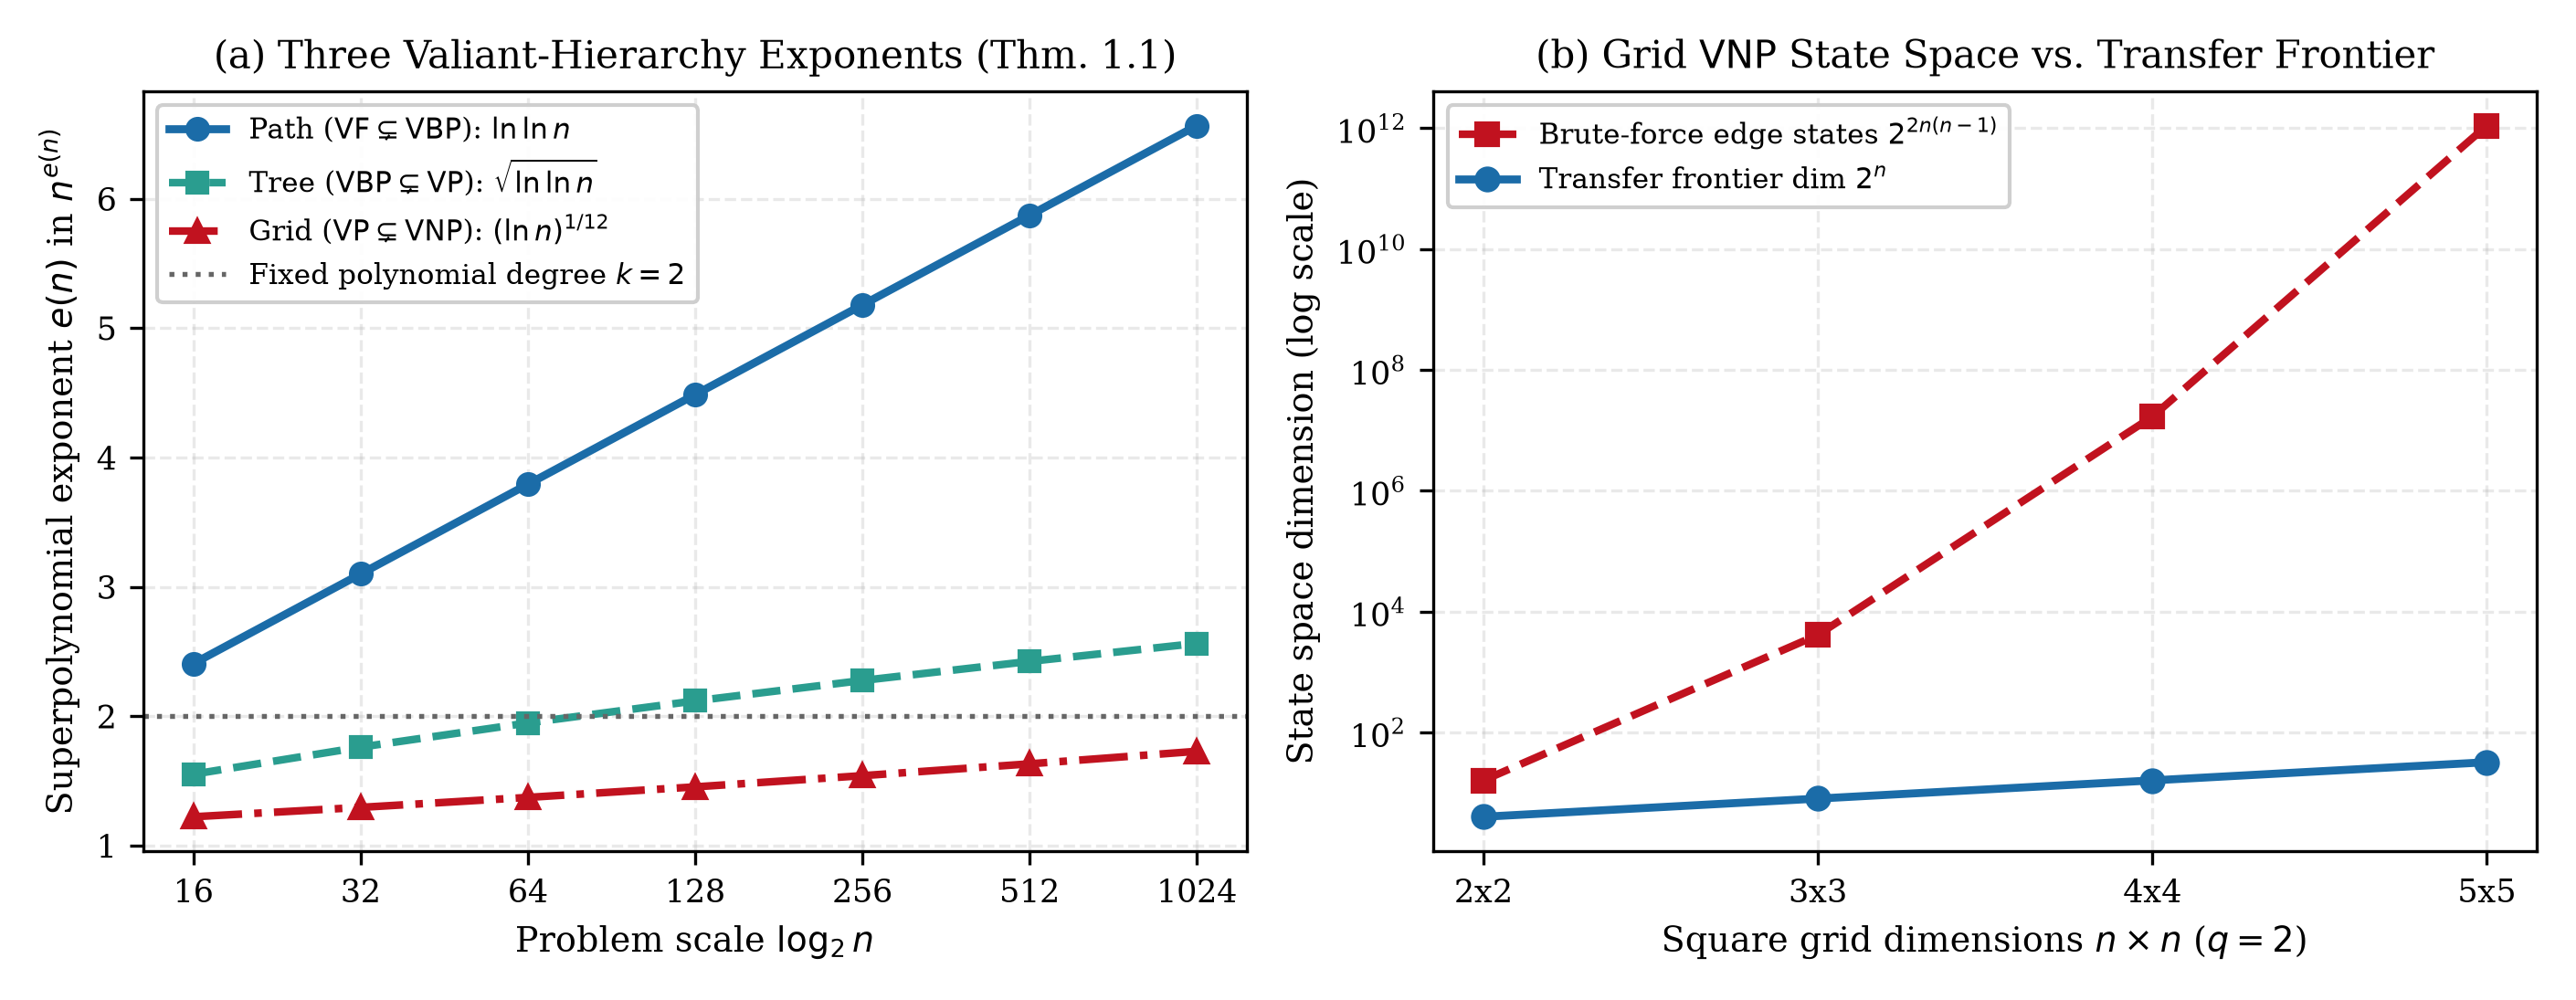
\includegraphics[width=0.90\linewidth]{figures/fig1_hierarchy_and_grid.png}
\caption{Valiant hierarchy exponents and grid state space. (a)~OpenAI Theorem~1.1 superpolynomial exponents ($\ln\ln n$, $\sqrt{\ln\ln n}$, $(\ln n)^{1/12}$) versus fixed polynomial degree $k=2$. (b)~Brute-force grid edge assignments $2^{2n(n-1)}$ versus exact transfer-matrix frontier dimension $2^n$.}
\label{fig:hier}
\end{figure}

\begin{figure}[t!]
\centering
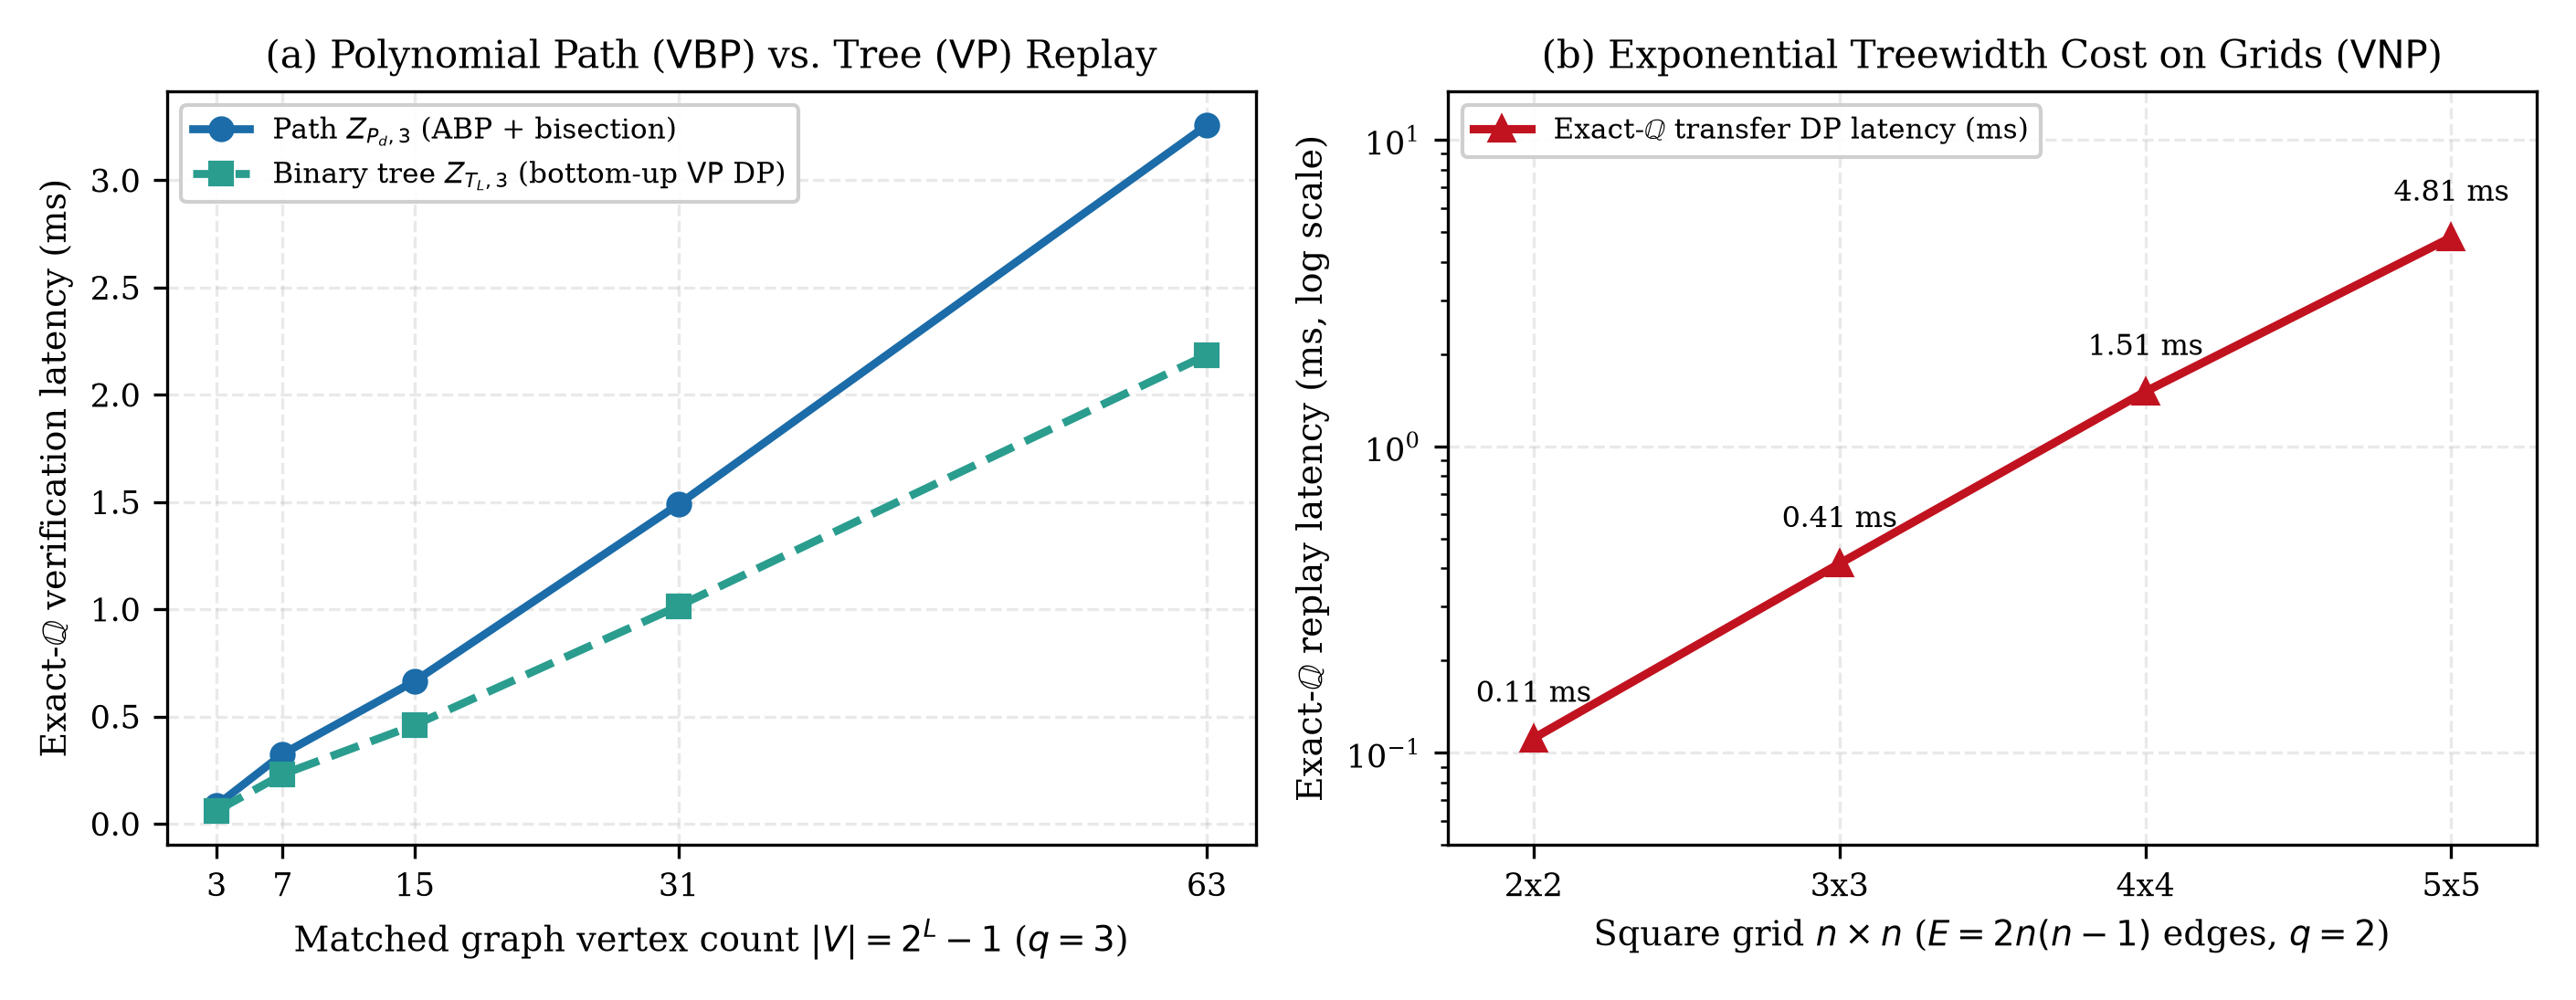
\includegraphics[width=0.90\linewidth]{figures/fig2_model_replay_scaling.png}
\caption{Exact-$\QQ$ model replay scaling. (a)~Matched-vertex polynomial verification times for paths ($\mathsf{VBP}$) and complete binary trees ($\mathsf{VP}$) at $q=3$. (b)~Exponential treewidth replay cost on $n\times n$ square grids ($2\times 2 \to 5\times 5$, $q=2$).}
\label{fig:scaling}
\end{figure}

\begin{figure}[t!]
\centering
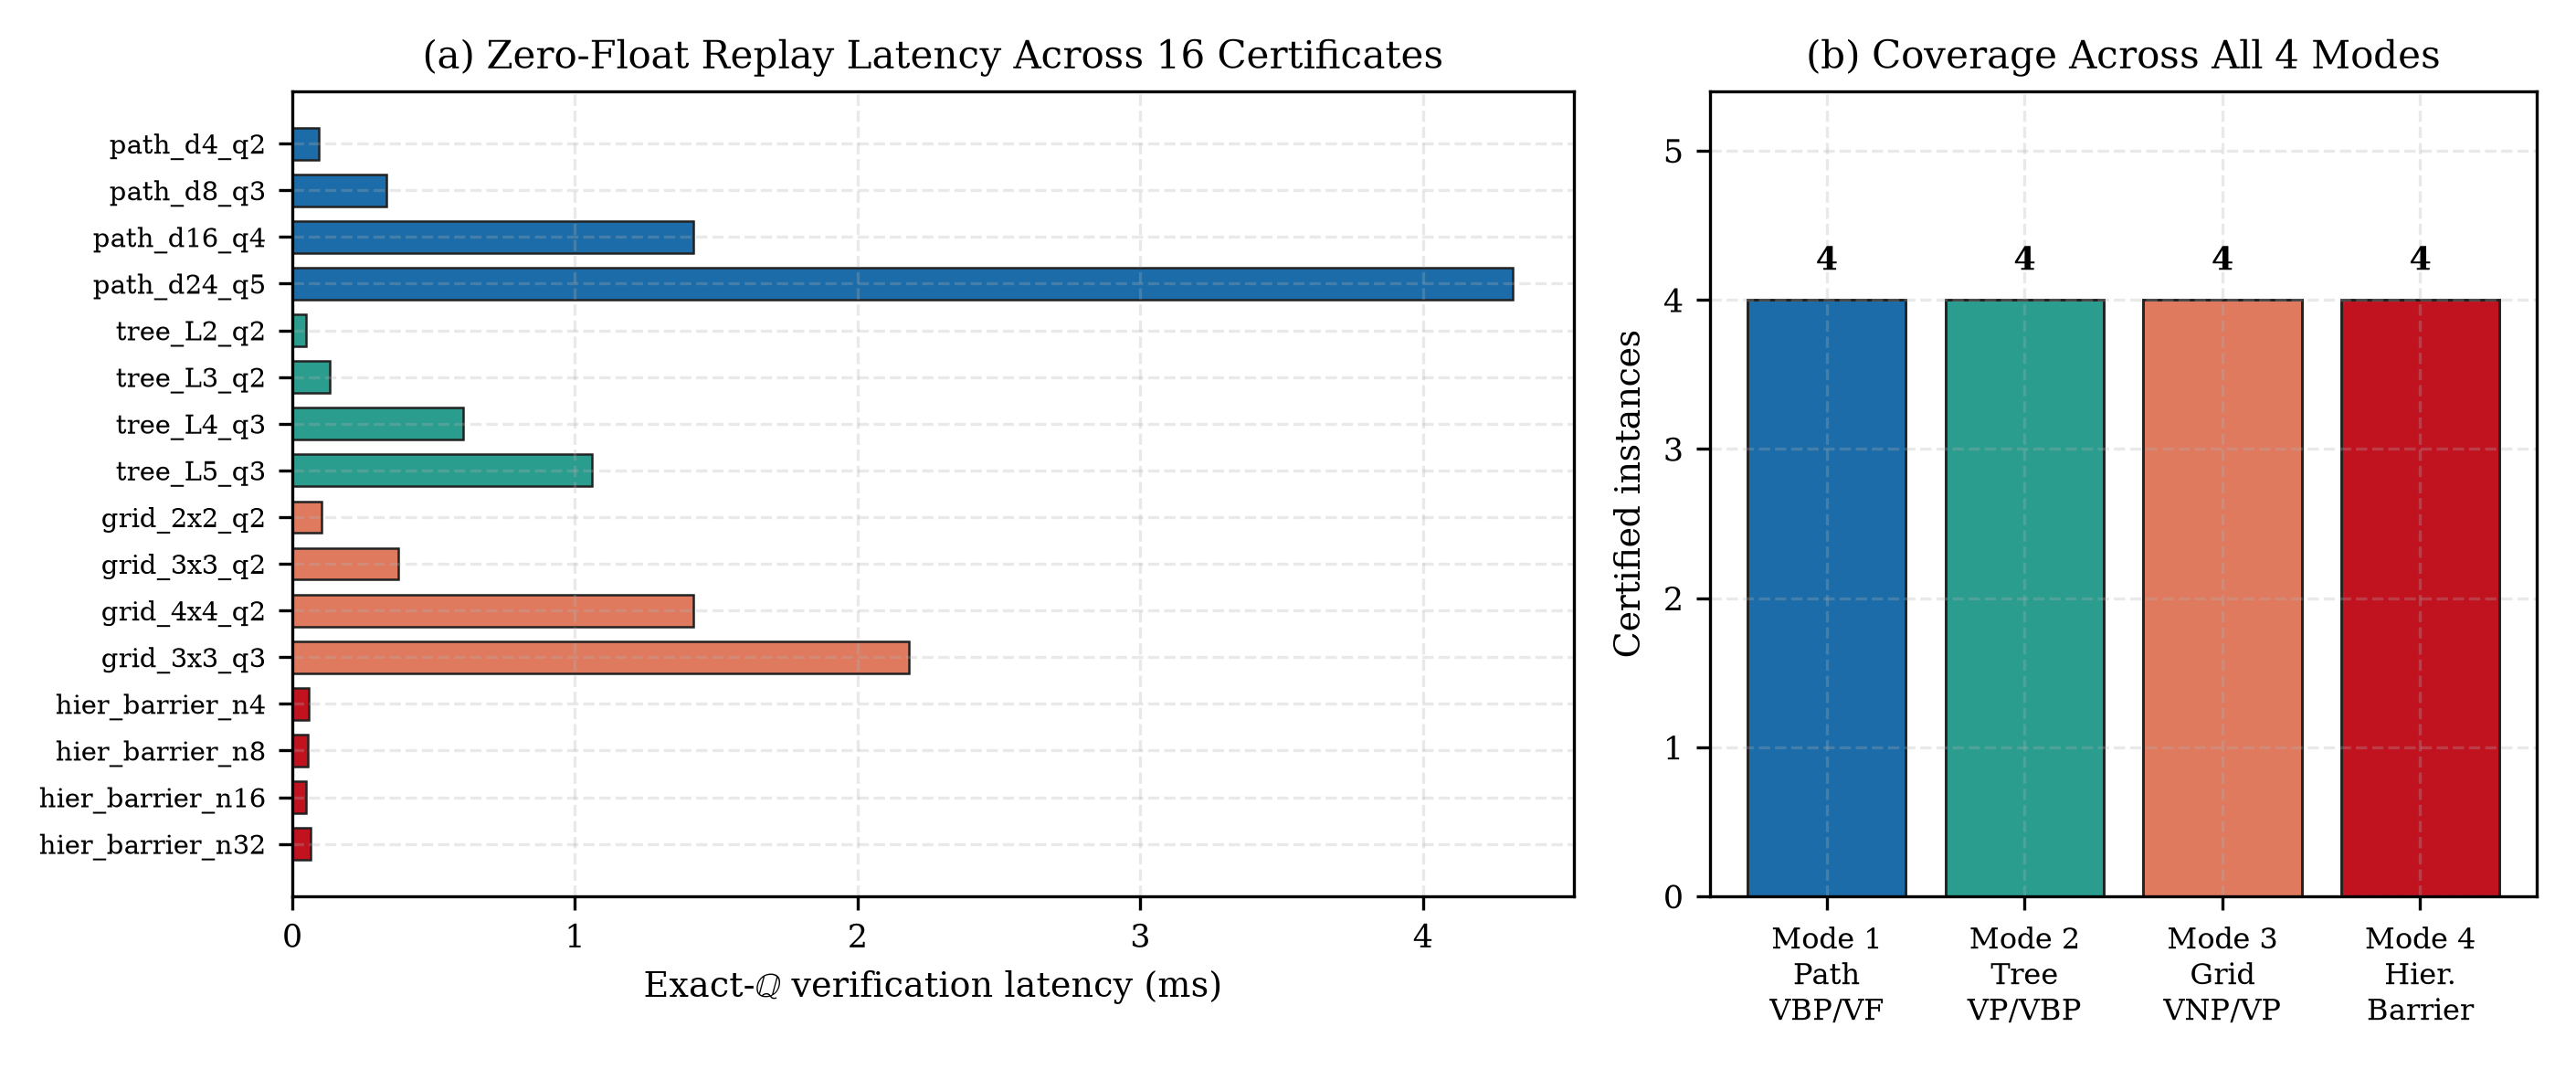
\includegraphics[width=0.90\linewidth]{figures/fig3_atlas_summary.png}
\caption{Certified atlas performance. (a)~Zero-float exact-$\QQ$ replay latencies across all $16$ \certschema{} certificates ($0.049$--$4.319\,\mathrm{ms}$). (b)~Balanced coverage ($4$ instances per mode) across all four certification modes.}
\label{fig:atlas}
\end{figure}

\section{Scope Boundaries and Outlook}\label{sec:outlook}

This work certifies exact finite-order path, binary-tree, and square-grid state sums, model-specific contraction equivalences, characteristic-free Boolean $\mathsf{VNP}$ selectors, and finite superpolynomial hierarchy chains over $\ZZ/\QQ$, rather than formalizing the full degree-component border-complexity lower-bound proofs or Euclidean tensor-price machinery of~\cite{openai2026hierarchy,openai2026vpvnp}. Extending \certschema{} to treewidth-bounded minor decompositions for arbitrary graph families is a natural next direction.

\bibliographystyle{plain}
\bibliography{references}

\end{document}
